
%
\documentclass[12pt]{article}     
\usepackage{graphicx}
\graphicspath{{figures/}}
\usepackage[top=2.5cm, bottom=2.5cm, left=3cm, right=3cm]{geometry}
\usepackage{titlesec}
\usepackage{longtable}
\usepackage[table,xcdraw]{xcolor}
\usepackage{todonotes}

\usepackage{float}

\usepackage[T2A,T1]{fontenc}
\usepackage[utf8]{inputenc}
\usepackage{csquotes}
\usepackage{tocloft}

\usepackage{amssymb} %For square itemized listss
\renewcommand{\labelitemi}{\tiny$\blacksquare$} %For square itemized lists

\usepackage{caption} 
\captionsetup{labelsep=period}

\usepackage{verbatimbox} %To put program code in the center using Verbatim

\titlelabel{\thetitle.\quad}

\usepackage{times}
\usepackage{fancyhdr}
\setlength{\parindent}{0cm}
\usepackage{setspace}
\onehalfspacing
%\usepackage{parskip}
\setlength{\parskip}{\baselineskip}
%\hangindent=0.7cm

\usepackage{amsmath} 
\usepackage{amsthm}
% Packages for building tables and tabulars 
\usepackage{array}
\usepackage{tabu}   % Wide lines in tables
\usepackage{xspace} % Non-eatable spaces in macros
\usepackage[colorlinks=true,linkcolor=blue]{hyperref}
\usepackage[all]{hypcap}
\usepackage{url}

% Packages for defining colourful text together with some colours
%\usepackage[table,xcdraw]{xcolor}
\definecolor{dkgreen}{rgb}{0,0.6,0}
\definecolor{gray}{rgb}{0.5,0.5,0.5}
\definecolor{mauve}{rgb}{0.58,0,0.82}
\definecolor{lightblue}{rgb}{0.95,0.97,1.0}
\definecolor{darkblue}{rgb}{0.90,0.92,1.0}

\usepackage{color}

% Standard package for drawing algorithms
% Since the thesis in article format we must define \chapter for
% the package algorithm2e (otherwise obscure errors occur) 
\let\chapter\section
\usepackage[ruled, vlined, linesnumbered]{algorithm2e}

% Macros that make sure that the math mode is set
\newcommand{\typeF}[1] {\ensuremath{\mathsf{type_{#1}}}\xspace}
\newcommand{\opDiv}{\ensuremath{\backslash \mathsf{div}}\xspace} 
\usepackage{listings}

\lstset{ 
  %language=python,                % the language of the code
  language=C++,
  basicstyle=\footnotesize,        % the size of the fonts that are used for the code
  %numbers=left,                   % where to put the line-numbers
  %numberstyle=\footnotesize,      % the size of the fonts that are used for the line-numbers
  numberstyle=\tiny\color{gray}, 
  stepnumber=1,                    % the step between two line-numbers. If it's 1, each line 
                                   % will be numbered
  numbersep=5pt,                   % how far the line-numbers are from the code
  backgroundcolor=\color{white},   % choose the background color. You must add \usepackage{color}
  showspaces=false,                % show spaces adding particular underscores
  showstringspaces=false,          % underline spaces within strings
  showtabs=false,                  % show tabs within strings adding particular underscores
  frame = lines,
  %frame=single,                   % adds a frame around the code
  rulecolor=\color{black},		   % if not set, the frame-color may be changed on line-breaks within 
                                   % not-black text (e.g. commens (green here))
  tabsize=2,                       % sets default tabsize to 2 spaces
  captionpos=b,                    % sets the caption-position to bottom
  breaklines=true,                 % sets automatic line breaking
  breakatwhitespace=false,         % sets if automatic breaks should only happen at whitespace
  %title=\lstname,                 % show the filename of files included with \lstinputlisting;
                                   % also try caption instead of title
                                   % also try caption instead of title
  keywordstyle=\color{blue},       % keyword style
  commentstyle=\color{dkgreen},    % comment style
  stringstyle=\color{mauve},       % string literal style
  escapeinside={\%*}{*)},          % if you want to add a comment within your code
  morekeywords={*,game, fun}       % if you want to add more keywords to the set
}

\usepackage{multirow}
\newcolumntype{C}[1]{>{\centering\let\newline\\\arraybackslash\hspace{0pt}}m{#1}}
\newcolumntype{L}[1]{>{\raggedright\let\newline\\\arraybackslash\hspace{0pt}}m{#1}}

\usepackage{booktabs,fixltx2e}
%\usepackage[flushleft]{threeparttable}
\usepackage{tikz}
%used for ex. for m prime
\usepackage{flexisym}
\usepackage{footnote}

\usepackage{arydshln}



\begin{document}

%------------------------------TIITELLEHT---------------------------------
\thispagestyle{fancy} %Leht sisaldab päist ja jalust
\renewcommand{\headrulewidth}{0pt} %Eemaldab päisest horisontaalse joone
\renewcommand{\footrulewidth}{0pt} %Eemaldab jalusest horisontaalse joone
\headheight = 57pt %Paneb paika päise laiuse (vastavalt kompilaatori soovitusele)
\footskip = 11pt %Jaluse ruum
\headsep = 0pt %Vähendab päise ja teksti vahelise kauguse nullini

\chead{ %Paigutab järgneva teksti päises keskele
 \textsc{\begin{Large} %Tekst suurtähtedega ja suuremaks
	Tallinn University of Technology\\
	\end{Large} }
	Department of Computer Science\\	
	TUT Centre for Digital Forensics and Cyber Security
}
\vspace*{7 cm} %Tekitab lehe alguse ja teksti vahele tühja ala vastava laiusega

\begin{center} %Tekst keskele
ITC70LT\\[0cm]

Christian Ponti 144704\\
\vspace{15pt}
\begin{LARGE}
\textsc{What approach can be used to gain network access from outside by using ICMPv6?\\}
\end{LARGE}
\vspace{10pt}
Master Thesis\\[2cm]
\end{center}

\begin{flushright} %Joondab teksti paremale
Supervisor: Bernhards Blumbergs\\[0cm]
PhD\\[0cm]
%[Ametinimetus]\\[0cm]
\end{flushright}

\cfoot{Tallinn 2016} %Lisab asukoha ja kuupäeva jalusesse
%\renewcommand{\headrulewidth}{0pt} %Eemaldab päisest horisontaalse joone
\pagebreak %Lehe lõpp

%---------------------------AUTORIDEKLARATSIOON-------------------------
\section*{\begin{center}
 Autorideklaratsioon
\end{center}}


Autorideklaratsioon on iga lõputöö kohustuslik osa, mis järgneb tiitellehele.
Autorideklaratsioon esitatakse järgmise tekstina:

Olen koostanud antud töö iseseisvalt. Kõik töö koostamisel kasutatud teiste autorite tööd, olulised seisukohad, kirjandusallikatest ja mujalt pärinevad andmed on viidatud. Käsolevat tööd ei ole varem esitatud kaitsmisele kusagil mujal.

Autor: [Ees$-$ ja perenimi]

[\today]
\pagebreak

%---------------------------ANNOTATION---------------------------------
\section*{\begin{center}
Annotatsioon
\end{center}}

Annotatsioon on lõputöö kohustuslik osa, mis annab lugejale ülevaate töö eesmärkidest, olulisematest käsitletud probleemidest ning tähtsamatest tulemustest ja järeldustest. Annotatsioon on töö lühitutvustus, mis ei selgita ega põhjenda midagi, küll aga kajastab piisavalt töö sisu. Inglisekeelset annotatsiooni nimetatakse Abstract, venekeelset aga


Sõltuvalt töö põhikeelest, esitatakse töös järgmised annotatsioonid:
\begin{itemize}
\item kui töö põhikeel on eesti keel, siis esitatakse annotatsioon eesti keeles mahuga $\frac{1}{2	}$ A4 lehekülge ja annotatsioon \textit{Abstract} inglise keeles mahuga vähemalt 1 A4 lehekülg;
\item kui töö põhikeel on inglise keel, siis esitatakse annotatsioon (Abstract)  inglise keeles mahuga $\frac{1}{2}$ A4 lehekülge ja annotatsioon eesti keeles mahuga vähemalt 1 A4 lehekülg;
\end{itemize}

Annotatsiooni viimane lõik on kohustuslik ja omab järgmist sõnastust:

Lõputöö on kirjutatud [mis keeles] keeles ning sisaldab teksti [lehekülgede arv] leheküljel, [peatükkide arv] peatükki, [jooniste arv] joonist, [tabelite arv] tabelit.
\pagebreak


%-----------------------------ABSTRACT-----------------------------------

\section*{\begin{center}
Abstract
\end{center}}
Võõrkeelse annotatsiooni koostamise ja vormistamise tingimused on esitatud eestikeelse annotatsiooni juures.

The thesis is in [language] and contains [pages] pages of text, [chapters] chapters, [figures] figures, [tables] tables.
\pagebreak

%---------------------Glossary of terms and Abbreviations---------------------

\section*{\begin{center}
Glossary of Terms and Abbreviations
\end{center}}
Lühendite  ning  mõistete  sõnastikku  lisatakse kõik töö põhitekstis kasutatud  uued  ning  ka mitmetähenduslikud üldtuntud terminid. Näiteks inglisekeelne lühend PC  võib tähendada nii Personal Computer kui ka Program Counter, sõltuvalt kontekstist. Lühendid ja mõisted esitatakse tabuleeritult kahte tulpa selliselt, et vasakul on esitatud lühend või mõiste ja paremal tulbas seletus. Inglisekeelsed sõnad seletustes esitatakse kaldkirjas. Alltoodud näited esitavad lühendite ja mõistete sõnastiku korrektset vormistamist.

\begin{tabular}{p{3 cm}ll} %tabel first column is 3cm.
IPv6&Internet Protocol version 6\\
ICMPv6&Internet Control Message Protocol version 6\\
Node&ll\\
NAT&dd\\
IANA&Internet Assigned Numbers Authority\\
BYID&Bring Your Own Device\\
OS&Operating System\\
IoT&Internet of Things\\
rootkit&ff
\end{tabular}
\pagebreak

%----------------------------SISUKORD----------------------------------
\tableofcontents
\newpage
%----------------------JOONISTE NIMEKIRI-------------------------------
\listoffigures
\pagebreak
%----------------------TABELITE NIMEKIRI---------------------------------
\listoftables
\pagebreak
%-----------------------------SISSEJUHATUS------------------------------- 
\section{Introduction}
\label{sec:1}


IPv6 is the designated successor of IPv4, a protocol specified and implemented in a context with a limited number of users and hosts, most of them circumscribed to the scientific world. The need of a new protocol arose 
because of a changed context: the evolution of new powerful devices and their spread in many field of the society, which in turn modified the behavior and the requests of new entities, being them individuals or big 
organizations. The new IP protocol has been specified and rewritten in many aspects, taking in consideration the evolution of the requirements and the future needs of the involved actors.\\
IPv6\cite{rfc2460}, with respect to his predecessor, changed in many aspects. The headers have been modified to accommodate new functionalities and improved capabilities, mainly it provides "expanded addressing 
capabilities", "header format simplification", "improved support for extensions and options", "flow labeling capability", and ``authentication and privacy capabilities". One of the most relevant aspect is the increased 
address space from 32 bits to 128 bits, which deals with the demand of new communicating devices to fulfill organization's requirements.\\
Despite IPv6 specifications have been formalized in 1998, its spread and adoption by the world community is far from being accomplished. Among the many possible reasons that could explain this behavior, two of them 
deserve particular attention. The first one is related to the lack of address space, which has been mitigated by the introduction of Network Address Translation (NAT)\cite{rfc3022}: the use of NAT allows to use a private, not routeable,
address space for the internal network of an organization, and the use of one, or limited number, public IPv4 address at the network boundary. This technique mitigated the need to introduce the 128 bits address space 
of IPv6, because organization's requirements to allocate new IPv4 address from IANA\footnote{\url{http://www.iana.org/}} have been reduced. The second reason is related to the applications and services offered by organizations. Networked 
applications have been written for, and tested against, IPv4. Many of them represents IT assets which are critical for the business assets and goals of enterprises: the introduction of new applications written for IPv6 
represents a great effort in terms of financial investment, time for implementation and testing, and use of enterprises' resources.\\
The IPv6 world is composed by a number of protocols, which are used by nodes to fulfill their requirements: some of them, with respect to their IPv4 version, have been obsoleted by new concepts and specifications of IPv6, 
while others have been rewritten with few changes. In this galaxy of protocols, one of them, present also in its version 4, deserves particular attention: ICMPv6.\\
ICMPv6, despite it shares almost the same naming convention with respect with the predecessor, could be considered a new protocol for a number of reasons, which make it a critical subject of research by the scientific 
community. The reasons behind its criticality arise because it holds a backward compatibility with the functions of its version 4, but at the same time it introduces a number of new functionalities, and responsibilities, 
for the correct behavior of an IPv6 node.\\
ICMPv4 has been used by IPv4 to manage error and informational messages to allow for a better management and troubleshooting of the network. While it is an important aspect of the network and it has been used by network 
administrators to manage network issues, it is not crucial for the correct working of the communication. This version has been tested for many years, with the identification of vulnerabilities which can be 
potentially be exploited by malicious actors. Many best practices\footnote{\url{http://www.cisco.com/c/en/us/support/docs/ip/access-lists/13608-21.html\#anc29}, accessed 20.03.2016}
\footnote{\url{http://www.cisco.com/c/en/us/about/security-center/firewall-best-practices.html\#\_Toc332805964}, accessed 20.03.2016} 
suggested to filter ICMPv4 messages at network boundaries to mitigate the risk of the exploitation of some vulnerabilities without 
compromising the network functionalities. Nowadays the network evolved in more sophisticated designs, and new concepts, like Bring Your Own Device (BYOD) and wireless networks, partially obsolete the very same concept of boundaries, bringing new 
threats to the internal network. The security controls could no more be applied only at the boundaries, but must be introduced in other segments of the network. This new security controls applies to the ICMPv4 protocol 
as well, and filtering must be introduced where such messages are not strictly required by network administrators.\\
“ICMPv6 is used by IPv6 nodes to report errors encountered in processing packets, and to perform other internet-layer functions, such as diagnostics (ICMPv6 ”ping”). ICMPv6 is an integral part of IPv6, and the base 
protocol (all the messages and behavior required by this specification) MUST be fully implemented by every IPv6 node.”\cite{rfc4443}\\
This paragraph of RFC 4443 describes broadly the purpose of ICMPv6, but the most important part is the last sentence, which states that the base protocol must be fully implemented by every IPv6 node. In the RFC 
terminology, the word “MUST, or the terms REQUIRED or SHALL, mean that the definition is an absolute requirement of the specification“\cite{rfc2119}. The real distinction between ICMPv4 and ICMPv6 in this context is formal: RFC 
792 states that ”ICMP ... must be implemented by every IP module“\cite{rfc792}, which means that an implementation is required. The ICMPv6 specification is more precise because it refers to every IPv6 node, which covers the 
implementation inside the module, but also, with the concept of node, implies that the node must be able to use its functionalities.\\
This is a fundamental distinction, because the best practices in use with ICMPv4, with ICMPv6 are no more relevant, at least with some message types. As it is written in this paper\cite{chak}, which cites RFC 4861\cite{rfc4861}, ”ICMPv6 is 
used for basic functionalities and used by other IPv6 protocols ... Neighbor Discovery Protocol is a protocol used with IPv6 to perform various tasks like router discovery, auto address configuration of a node, neighbor 
discovery, Duplicate Address Detection, determining the Link Layer addresses of other nodes, address prefix discovery, and maintaining routing information about the paths to other active neighbor nodes“.\\
This is the first critical point to consider: version 4 and version 6 of the ICMP protocol share some functionalities, but are different protocols. ICMPv6 is not a protocol modified to adapt itself to IPv6, a new analysis 
must be performed in an exhaustive way taking into account new scenarios, and new best practices must be applied to mitigate the risk of exploitation of new vulnerabilities related to its functionalities.\\
Another important aspect to take into consideration when dealing with IPv6 in general, and with ICMPv6, is the transition from version 4 to version 6. For the aforementioned reasons mentioned, many organizations 
delayed as much as they could the deployment of a full IPv6 network. Nevertheless the scientific community continued to improve the new version and its related protocols, and Operating Systems (OS) started to include 
them in their network implementations. At the same time, techniques to allow a slow transition have been developed: examples of that are the dual stack, the presence and coexistence of both protocol versions in the same 
node, or the encapsulation of IPv6 inside IPv4, in those network segments where IPv6 has not been deployed yet. In addition, in many OS, IPv6 is active by default and preferred over IPv4.\\
These aspects must not be underestimated and show again how critical and urgent is an in-depth analysis of ICMPv6: not only this protocol is fundamental for IPv6 and the best practices can be used only against the old 
version, but it is already present and activated in OS that users employ in their everyday life. This last distinction is very important because it introduces another aspect to take into account: network 
administrator and security officer must not deal only with threats deriving from the exploitation of technical vulnerabilities, but also with behavioral procedures shaped around years of practice. IPv6 and ICMPv6 are 
not protocol that will be introduced in the future, they are already present in this transition period and we must deal with them now. Countermeasures must be in place, at the network boundaries and inside critical 
network segments above all, that take into consideration version 6 of the protocols. Such countermeasures must follow new best practices carefully shaped around the new version.\\
The underlined elements, the differences between the two ICMP version and the transition period with the coexistence of IPv4 and IPv6, lead to another topic: the impact of the full deployment of IPv6, and ICMPv6, and the 
implications for the involved actors, being them users, enterprises, states, or malicious actors.\\
The scientific community has been involved in the specification, in the improvement, and testing of the protocols since time. But, with respect with the preceding version of the protocols, version 6 of the suite 
must deal with a very different situation. The electronic communication is spread around the world in a pervasive way, and the near future, with the Internet of Things (IoT)
\footnote{IoT, \url{http://www.theinternetofthings.eu/what-is-the-internet-of-things}, accessed 21.03.2016}, will further the spread. ICMPv6, and IPv6, 
will be fully deployed in a world strongly dependent on the electronic communication, where critical infrastructures (CI) must be managed and protected, where enterprises relies on its IT infrastructure to support their business 
assets, and where users are tight to their online experience for their everyday needs. This change in the very basic infrastructure of the network will have an impact which has no terms of comparison with respect to IPv4, 
whose slow deployment allowed to discover the concept of security and to learn by experience. The transition period, which introduced some security issues, in this case works as a mitigation technique to allow researcher 
to test the protocols in an exhaustive way, without waiting that the fully deployed IPv6 infrastructures reveals potential weaknesses.\\
This urgency can be better understood by taking into consideration the evolution of the threats, the sophistication of malware, and the malicious actors involved in the research of vulnerabilities to exploit, as well as 
their purposes and means to reach their goals.\\
The term Advanced Persistent Threat (APT) is used to define ''any sophisticated adversary engaged in information warfare in support of long-term strategic goals``\cite{apt}. One of the main characteristic of APT detected 
in the wild is the sophistication of the attack. One example is the Uroburos rootkit\cite{uroburos}, which ''modular structure allows extending it with new features easily, which makes it not only highly sophisticated 
but also highly flexible and dangerous``. The analysis of the rootkit suggests that ''the development of a framework like Uroburos is a huge investment`` and ''that it was designed to target government institutions, 
research institutions or companies dealing with sensitive information as well as similar high-profile targets``. There are other example of APT that suggested an evolution of the threat landscape, like Stuxnet\cite{stuxnet}.
Even if the aforementioned APT do not target directly IPv6, they share a common characteristic which is important to underline: the sophistication, the investment behind them, and the presence of an Advanced Persistent 
Adversary (APA)\cite{apa}, term that ''depicts not only the threat, but the threat actors as well``.\\
The evolution of the threat landscape depicts a situation where APA, often associated with groups sponsored by state actors, have unlimited budget to develop very sophisticated attacks to reach their goals. In the current 
situation, given the impact that the full deployment of IPv6 will have, those actors have the resources and the motivation to research and discover vulnerabilities in IPv6, ICMPv6, and other protocols involved. 
Moreover, if this research will succeed, APA can gain a considerable advantage over their opponents, because a possible vulnerability at network layer may allow to bypass more easily the security mechanisms in place and 
give more robust mechanisms to stay undetected for longer.\\
While research and tests on ICMPv6 are an ongoing process, the urgency and criticality of the subject require a more in-depth analysis which take into account the full deployment, but also the transition period. To 
pursue this goal it is important to start from the specifications of the protocol, the RFCs. Those documents represent a guideline, the result of an agreement between many stakeholders. As a guideline, there is no 
guarantee that the implementation will follow the suggestion, even in the sections specified with a ''must``.\\
It is worth to underline the contribution of this research, which start by producing the necessary awareness with regard to IPv6 and ICMPv6. This is the starting point to understand the need to analyze the protocols in 
detail. Furthermore, it is important to see the big picture, which include not only ICMPv6, but also its relationship with the devices involved in the communication, the target hosts, and the firewalls through which the 
packets must transit. Firewalls are devices configured by human beings, which may commit mistakes and use different best practices. Each configuration can produce a different scenario, which is worth to analyze because 
in the real world each system may differ from another, and the goal of an APA is to find these slight differences between them to take advantage. A scenario-based experiment needs also a test set, based on RFC specifications,
and the implementation of a software to conduct the experiments.\\
The next chapters of this work will explore the backgrounds, the specification inside RFCs, and the related work(see~\ref{sec:2}), which includes existing tools and projects to test ICMPv6, and a review of the literature.
Then the analysis proceeds with definition of the methodology(see~\ref{sec:3}) of this research, which is based on the scientific method of the experimentation; the chapter includes the motivation behind this choice and 
behind the choice of the technology to conduct the experiments. The implementation is the next chapter(see~\ref{sec:4}), which deal with the details of the technology, followed by the experiment(see~\ref{sec:5}), which 
describes the set of performed tests. The chapter related to the results(see~\ref{sec:6}) includes a discussion about the results of the experiment and its meaning. Finally, the conclusions(see~\ref{sec:7}) summarizes the 
research, discuss about suggestions and future work.

 

\pagebreak
%------------------------------BACKGROUND AND RELATED WORK-----------------------------------
\section{Background and Related Work}
\label{sec:2}


\subsection{Background}
\label{sub:background}

''The Internet Standards process is an activity of the Internet Society that is organized and managed on behalf of the Internet community by the Internet Architecture Board (IAB)\footnote{\url{https://www.iab.org/}} and 
the Internet Engineering Steering 
Group (IESG)\footnote{\url{https://www.ietf.org/iesg/}}.
... an Internet Standard is a specification that is stable and well-understood, is technically competent, has multiple, independent, and interoperable implementations with substantial operational experience, 
enjoys significant public support, and is recognizably useful in some or all parts of the Internet. ... Each distinct version of an Internet standards-related specification is published as part of the "Request for 
Comments" (RFC) document series.  This archival series is the official publication channel for Internet standards documents and other publications of the IESG, IAB, and Internet community.``\cite{rfc2026}\\

This work starts by analyzing the RFCs related to ICMPv6, which specify the protocol and the features to which each implementation must adhere. The main goal of an agreement on a protocol is interoperability
\footnote{\url{http://www.merriam-webster.com/dictionary/interoperability}}, but, since this is not a binding process, and even though implementations follow the main specifications, it is always possible that some of 
them do not adhere completely. This could lead to some interoperability issues, which may introduce vulnerabilities in the protocol.\\
The background of this research is represented by two RFCs, ''Internet Control Message Protocol (ICMPv6) for the Internet Protocol Version 6 (IPv6) Specification``\cite{rfc4443}, and ''Neighbor Discovery for IP version 6 
(IPv6)``\cite{rfc4861}. These two RFCs specify the general header for ICMPv6 messages, and each specific message header to which each implementation must adhere.\\
The IPv6 specification\cite{rfc2460} is only partially in the scope of this research, but it must be mentioned, because of its tight relationship with ICMPv6, and because in each ICMPv6 message type specification some of 
its fields are cited, as it will be underlined later in the chapter.


\subsubsection{Terminology}
\label{subsub:terminology}

This research background's analysis starts from the terminology, since it is important to define and understand the terms which will be spread across the RFCs. The definition's sources are the RFCs.

\begin{tabular}{L{3.3cm}L{11.2cm}}
\hdashline
\textit{Node}:&a device that implements IPv6.\\
\hdashline
\textit{Link}:&a communication facility or medium over which nodes can communicate at the link layer, i.e., the layer immediately below IPv6.\\
\hdashline
\textit{Interface}:&a node's attachment to a link.\\
\hdashline
\textit{Neighbors}:&nodes attached to the same link.\\
\hdashline
\textit{Prefix}:&a bit string that consists of some number of initial bits of an address.\\
\hdashline
\textit{On-link}:&an address that is assigned to an interface on a specified link.\\
\hdashline
\textit{Off-link}:&an address that is not assigned to any interfaces on the specified link.\\
\hdashline
\textit{Longest prefix match}:&the process of determining which prefix in a set of prefixes covers a target address. A target address is covered by a prefix if all of the bits in the prefix match the left-most 
bits of the target address. When multiple prefixes cover an address, the longest prefix is the one that matches.\\
\hdashline
\textit{Reachability}:&whether or not the one-way "forward" path to a neighbor is functioning properly. In particular, whether packets sent to a neighbor are reaching the IP layer on the neighboring machine and are 
being processed properly by the receiving IP layer.\\
\hdashline
\textit{Packet}:&an IPv6 header plus payload.\\
\hdashline
\textit{Link MTU}:&the maximum transmission unit, i.e., maximum packet size in octets, that can be conveyed over a link.\\
\hdashline
\textit{Path MTU}:&the minimum link MTU of all the links in a path between a source node and a destination node.\\
\hdashline
\textit{Multicast capable}:&a link that supports a native mechanism at the link layer for sending packets to all (i.e., broadcast) or a subset of all neighbors.\\
\hdashline
\textit{Point-to-point}:&a link that connects exactly two interfaces.\\
\hdashline
\end{tabular}

\begin{tabular}{L{3.3cm}L{11.2cm}}
\hdashline
\textit{Link-local address}:&a unicast address having link-only scope that can be used to reach neighbors.\\
\hdashline
\textit{All-nodes multicast address}:&the link-local scope address to reach all nodes, FF02::1.\\
\hdashline
\textit{All-routers multicast address}:&the link-local scope address to reach all routers, FF02::2.\\
\hdashline
\textit{Solicited-node multicast address}:&a link-local scope multicast address that is computed as a function of the solicited target's address. The function is chosen so that IP addresses that differ only in the most 
significant bits will map to the same solicited-node address thereby reducing the number of multicast addresses a node must join at the link layer.\\
\hdashline
\end{tabular}


\subsubsection{RFC 2460}
\label{subsub:2460}
The table (see~\ref{table:IPv6}) shows the specification of the IPv6 header. From the point of view of this research, there are four interesting fields which are strictly involved in the ICMPv6 specification:
\vspace{-15pt}
\begin{itemize}
 \item \textbf{Next Header}:\quad 8-bit, identifies the type of header immediately following the IPv6 header. Uses the same values as the IPv4 Protocol field. The ICMPv6 value is 58. The complete list is available on 
 IANA's website\footnote{\url{http://www.iana.org/assignments/protocol-numbers/protocol-numbers.xhtml}, accessed on 27.03.2016}
 \item \textbf{Hop Limit}:\quad 8-bit, decremented by 1 by each node that forwards the packet. The packet is discarded if Hop Limit is decremented to zero.
 \item \textbf{Source Address}:\quad 128-bit address of the originator of the packet.
 \item \textbf{Destination Address}:\quad 128-bit address of the intended recipient of the packet.
\end{itemize}

\vspace{25pt}
\begin{savenotes}
\begin{table}[h]
\centering
\begin{tabular}{|C{1.5cm}C{1.5cm}C{1.5cm}C{1.5cm}C{1.5cm}C{1.5cm}C{1.5cm}C{1.5cm}|}
\hline
\multicolumn{1}{|C{1.5cm}}{\cellcolor{darkblue} Version}&\multicolumn{2}{|C{3.0cm}|}{\cellcolor{lightblue} Traffic Class}&\multicolumn{5}{C{7.5cm}|}{\cellcolor{darkblue} Flow Label}\\
\hline
\multicolumn{4}{|C{6.0cm}}{\cellcolor{lightblue} Payload Length}&\multicolumn{2}{|C{3.0cm}|}{\cellcolor{darkblue} Next Header}&\multicolumn{2}{C{3.0cm}|}{\cellcolor{lightblue} Hop Limit}\\
\hline
\rowcolor{darkblue}
\multicolumn{8}{|c|}{}\\
\rowcolor{darkblue}
\multicolumn{8}{|c|}{}\\
\rowcolor{darkblue}
\multicolumn{8}{|c|}{}\\
\rowcolor{darkblue}
\multicolumn{8}{|c|}{\multirow{-4}{*}{\hfil Source Address}}\\
\hline
\rowcolor{lightblue}
\multicolumn{8}{|c|}{}\\
\rowcolor{lightblue}
\multicolumn{8}{|c|}{}\\
\rowcolor{lightblue}
\multicolumn{8}{|c|}{}\\
\rowcolor{lightblue}
\multicolumn{8}{|c|}{\multirow{-4}{*}{\hfil Destination Address}}\\
\hline
\end{tabular}
\caption{IPv6 Header}
\label{table:IPv6}
\end{table}
\end{savenotes}

\subsubsection{RFC 4443}
\label{subsub:4443}

The Internet Control Message Protocol (ICMPv6) for the Internet Protocol Version 6 (IPv6) Specification categorizes two broad type of messages, error and informational messages.\\
As shown in the table (see~\ref{table:ICMPv6}), the general ICMPv6 header format is composed by an 8 bit \textbf{type} field, an 8 bit \textbf{code} field, and a 16 bit \textbf{checksum} field. The message body suggests 
specific header fields which are characteristic of each message type.\\
ICMPv6 messages are categorized by its type field, while the code field in this specification identifies a specific message under the category.

Error messages are characterized by a 0 in the high order bits of the type field, which gives a value range between 0 and 127. informational message are instead characterized by a 1 in the high order bits, for a possible 
value range between 128 and 255.

\vspace{20pt}
\begin{savenotes}
\begin{table}[h]
\centering
\begin{tabular}{|C{1.5cm}C{1.5cm}C{1.5cm}C{1.5cm}C{1.5cm}C{1.5cm}C{1.5cm}C{1.5cm}|}
\hline
\multicolumn{2}{|C{3.0cm}}{\cellcolor{darkblue} Type}&\multicolumn{2}{|C{3.0cm}|}{\cellcolor{lightblue} Code}&\multicolumn{4}{C{6.0cm}|}{\cellcolor{darkblue} Checksum}\\
\hline
\rowcolor{lightblue}
\multicolumn{8}{|c|}{}\\
\rowcolor{lightblue}
\multicolumn{8}{:c:}{\multirow{-2}{*}{\hfil Message Body}}\\
\hdashline
%\hline
\end{tabular}
\caption{ICMPv6 General Header Format}
\label{table:ICMPv6}
\end{table}
\end{savenotes}

\vspace{30pt}
The next two table (see~\ref{table:ICMPv6ErrorMessages} and~\ref{table:ICMPv6InformationalMessages}) summarize the type of ICMPv6 messages described in this RFC.\\

\textbf{ICMPv6 Error Messages}\\
\begin{savenotes}
\begin{table}[h]
\centering
\begin{tabular}{|L{3.0cm}|L{8.0cm}|}
\rowcolor{lightblue}
\hline
Type field&Error Message\\
\hline
1&Destination Unreachable\\
\hline
2&Packet Too Big\\
\hline
3&Time Exceeded \\
\hline
4&Parameter Problem\\
\hline
100&Private experimentation\\
\hline
101&Private experimentation\\
\hline
127&Reserved for expansion of ICMPv6 error messages\\
\hline
\end{tabular}
\caption{ICMPv6 Error Messages}
\label{table:ICMPv6ErrorMessages}
\end{table}
\end{savenotes}

\textbf{ICMPv6 Informational Messages}\\
\begin{savenotes}
\begin{table}[h]
\centering
\begin{tabular}{|L{3.0cm}|L{8.0cm}|}
\rowcolor{lightblue}
\hline
Type field&Informational Message\\
\hline
128&Echo Request\\
\hline
129&Echo Reply\\
\hline
200&Private experimentation\\
\hline
201&Private experimentation\\
\hline
255&Reserved for expansion of ICMPv6 informational messages\\
\hline
\end{tabular}
\caption{ICMPv6 Informational Messages}
\label{table:ICMPv6InformationalMessages}
\end{table}
\end{savenotes}

The RFC, besides ICMPv6 fields, gives directives also for IPv6 fields of interest. For all the error messages and Echo Reply is the Destination Address field, which is ''copied from the Source Address field of the 
invoking packet``. For an Echo Request, the IPv6 field is ''any legal IPv6 address``. 


\textbf{Destination Unreachable}

The first inspected message type is Destination Unreachable. Its purpose is to generate an error ''in response to a packet that cannot be delivered to its destination address for reasons other than congestion``.\\
The table (see~\ref{table:destUnreach}) shows the header fields.

\begin{savenotes}
\begin{table}[h]
\centering
\begin{tabular}{|C{1.5cm}C{1.5cm}C{1.5cm}C{1.5cm}C{1.5cm}C{1.5cm}C{1.5cm}C{1.5cm}|}
\hline
\multicolumn{2}{|C{3.0cm}}{\cellcolor{darkblue} Type}&\multicolumn{2}{|C{3.0cm}|}{\cellcolor{lightblue} Code}&\multicolumn{4}{C{6.0cm}|}{\cellcolor{darkblue} Checksum}\\
\hline
\rowcolor{lightblue}
\multicolumn{8}{|c|}{Unused}\\
\hline
\rowcolor{darkblue}
\multicolumn{8}{|c|}{}\\
\rowcolor{darkblue}
\multicolumn{8}{:c:}{\multirow{-2}{*}{\parbox{10cm}{As much of invocking packet as possible without the ICMPv6 packet exceeding the minimum IPv6 MTU}}}\\
\hdashline
\end{tabular}
\caption{Destination Unreachable}
\label{table:destUnreach}
\end{table}
\end{savenotes}

The table (see~\ref{table:destUnreachCodes}) summarizes the type, which is always 1, and code fields of the header, with the corresponding code name of the message.\\
\begin{savenotes}
\begin{table}[h]
\centering
\begin{tabular}{|L{2.0cm}|L{2.0cm}|L{6.0cm}|}
\rowcolor{lightblue}
\hline
Type&Code&Description\\
\hline
\multirow{7}{*}{1}&0&No Route to Destination\\ \cline{2-3}
&1&Communication with destination administratively prohibited\\ \cline{2-3}
&2&Beyond scope of source address\\ \cline{2-3}
&3&Address unreachable\\ \cline{2-3}
&4&Port unreachable\\ \cline{2-3}
&5&Source address failed ingress/egress policy\\ \cline{2-3}
&6&Reject route to destination\\ \cline{2-3}
\hline
\end{tabular}
\caption{Destination Unreachable Codes}
\label{table:destUnreachCodes}
\end{table}
\end{savenotes}

The Unused field accordingly to the RFC must be initialized to zero by the originator and ignored by the receiver.\\
The following illustrates the meaning behind codes and description:

\textbf{No Route to Destination}: lack of a matching entry in the forwarding node's routing table\\
\textbf{Communication with destination administratively prohibited}: administrative prohibition (e.g., a "firewall filter")\\
\textbf{Beyond scope of source address}: the destination is beyond the scope of the source address (e.g., when a packet has a link-local source address and a global-scope destination address)\\
\textbf{Address unreachable}: the reason for the failure to deliver cannot be mapped to any of other codes\\
\textbf{Port unreachable}: generated in response to a packet for which the transport protocol (e.g., UDP) has no listener\\
\textbf{Source address failed ingress/egress policy}: the packet with this source address is not allowed due to ingress or egress filtering policies\\
\textbf{Reject route to destination}: the route to the destination is a reject route (may occur if the router has been configured to reject all the traffic for a specific prefix).\\

\textbf{Packet Too Big}

A Packet Too Big must be sent by a router in response to a packet that it cannot forward because the packet is larger than the MTU of the outgoing link.\\
The table (see~\ref{table:packettoobig}) shows the header fields.\\

\begin{savenotes}
\begin{table}[h]
\centering
\begin{tabular}{|C{1.5cm}C{1.5cm}C{1.5cm}C{1.5cm}C{1.5cm}C{1.5cm}C{1.5cm}C{1.5cm}|}
\hline
\multicolumn{2}{|C{3.0cm}}{\cellcolor{darkblue} Type}&\multicolumn{2}{|C{3.0cm}|}{\cellcolor{lightblue} Code}&\multicolumn{4}{C{6.0cm}|}{\cellcolor{darkblue} Checksum}\\
\hline
\rowcolor{lightblue}
\multicolumn{8}{|c|}{MTU}\\
\hline
\rowcolor{darkblue}
\multicolumn{8}{|c|}{}\\
\rowcolor{darkblue}
\multicolumn{8}{:c:}{\multirow{-2}{*}{\parbox{10cm}{As much of invocking packet as possible without the ICMPv6 packet exceeding the minimum IPv6 MTU}}}\\
\hdashline
\end{tabular}
\caption{Packet Too Big}
\label{table:packettoobig}
\end{table}
\end{savenotes}

For this message the type field must always be 2 and the code set to 0 and ignored by the receiver. The MTU value represent ''the Maximum Transmission Unit of the next-hop link``.


\textbf{Time Exceeded Message}

The first table (see~\ref{table:timeExceeded}) underlines the header fields of this type of message, while the second one (see~\ref{table:timeExceededCodes}) shows the codes.
\begin{savenotes}
\begin{table}[h]
\centering
\begin{tabular}{|C{1.5cm}C{1.5cm}C{1.5cm}C{1.5cm}C{1.5cm}C{1.5cm}C{1.5cm}C{1.5cm}|}
\hline
\multicolumn{2}{|C{3.0cm}}{\cellcolor{darkblue} Type}&\multicolumn{2}{|C{3.0cm}|}{\cellcolor{lightblue} Code}&\multicolumn{4}{C{6.0cm}|}{\cellcolor{darkblue} Checksum}\\
\hline
\rowcolor{lightblue}
\multicolumn{8}{|c|}{Unused}\\
\hline
\rowcolor{darkblue}
\multicolumn{8}{|c|}{}\\
\rowcolor{darkblue}
\multicolumn{8}{:c:}{\multirow{-2}{*}{\parbox{10cm}{As much of invocking packet as possible without the ICMPv6 packet exceeding the minimum IPv6 MTU}}}\\
\hdashline
\end{tabular}
\caption{Time Exceeded}
\label{table:timeExceeded}
\end{table}
\end{savenotes}

If a router receives a packet with a Hop Limit of zero, or if a router decrements a packet's Hop Limit to zero, it must discard the packet and originate an ICMPv6 Time Exceeded message with Code 0 to the source of the 
packet. An ICMPv6 Time Exceeded message with Code 1 is used to report fragment reassembly timeout.\\

\begin{savenotes}
\begin{table}[h]
\centering
\begin{tabular}{|L{2.0cm}|L{2.0cm}|L{6.0cm}|}
\rowcolor{lightblue}
\hline
Type&Code&Description\\
\hline
\multirow{2}{*}{3}&0&Hop limit exceeded in transit\\ \cline{2-3}
&1&Fragment reassembly time exceeded \\ \cline{2-3}
\hline
\end{tabular}
\caption{Time Exceeded Codes}
\label{table:timeExceededCodes}
\end{table}
\end{savenotes}


\textbf{Parameter Problem Message}

''If an IPv6 node processing a packet finds a problem with a field in the IPv6 header or extension headers such that it cannot complete processing the packet, it must discard the packet and should originate an ICMPv6 
Parameter Problem message to the packet's source, indicating the type and location of the problem``.\\
The table (see~\ref{table:paramProb}) underlines the header fields of this type of message.\\

\begin{savenotes}
\begin{table}[h]
\centering
\begin{tabular}{|C{1.5cm}C{1.5cm}C{1.5cm}C{1.5cm}C{1.5cm}C{1.5cm}C{1.5cm}C{1.5cm}|}
\hline
\multicolumn{2}{|C{3.0cm}}{\cellcolor{darkblue} Type}&\multicolumn{2}{|C{3.0cm}|}{\cellcolor{lightblue} Code}&\multicolumn{4}{C{6.0cm}|}{\cellcolor{darkblue} Checksum}\\
\hline
\rowcolor{lightblue}
\multicolumn{8}{|c|}{Pointer}\\
\hline
\rowcolor{darkblue}
\multicolumn{8}{|c|}{}\\
\rowcolor{darkblue}
\multicolumn{8}{:c:}{\multirow{-2}{*}{\parbox{10cm}{As much of invocking packet as possible without the ICMPv6 packet exceeding the minimum IPv6 MTU}}}\\
\hdashline
\end{tabular}
\caption{Parameter Problem}
\label{table:paramProb}
\end{table}
\end{savenotes}

The table (see~\ref{table:paramProbCodes}) shows a mapping between each code and a description of the error.
\begin{savenotes}
\begin{table}[h]
\centering
\begin{tabular}{|L{2.0cm}|L{2.0cm}|L{6.0cm}|}
\rowcolor{lightblue}
\hline
Type&Code&Description\\
\hline
\multirow{3}{*}{4}&0&Erroneous header field encountered\\ \cline{2-3}
&1&Unrecognized Next Header type encountered\\ \cline{2-3}
&2&Unrecognized IPv6 option encountered \\
\hline
\end{tabular}
\caption{Parameter Problem Codes}
\label{table:paramProbCodes}
\end{table}
\end{savenotes}

Accordingly to the specification, the pointer field ''identifies the octet offset within the invoking packet where the error was detected. The pointer will point beyond the end of the ICMPv6 packet if the field in error 
is beyond what can fit in the maximum size of an ICMPv6 error message``.\\

\textbf{Echo Request}

The RFC states that each node must implements an Echo mechanism in order to produce Echo Requests and answer with Echo Replies. It also mentions the implementation of an application layer interface, for diagnostics 
purposes, to originate requests and receive replies.\\
The table (see~\ref{table:echoReq}) shows the header fields of an Echo Request message.\\

\begin{savenotes}
\begin{table}[h]
\centering
\begin{tabular}{|C{1.5cm}C{1.5cm}C{1.5cm}C{1.5cm}C{1.5cm}C{1.5cm}C{1.5cm}C{1.5cm}|}
\hline
\multicolumn{2}{|C{3.0cm}}{\cellcolor{darkblue} Type}&\multicolumn{2}{|C{3.0cm}|}{\cellcolor{lightblue} Code}&\multicolumn{4}{C{6.0cm}|}{\cellcolor{darkblue} Checksum}\\
\hline
\multicolumn{4}{|c|}{\cellcolor{lightblue} Identifier}&\multicolumn{4}{c|}{\cellcolor{darkblue} Sequence Number}\\
\hline
\rowcolor{lightblue}
\multicolumn{8}{|c|}{}\\
\rowcolor{lightblue}
\multicolumn{8}{:c:}{\multirow{-2}{*}{\hfil Data}}\\
\hdashline
\end{tabular}
\caption{Echo Request}
\label{table:echoReq}
\end{table}
\end{savenotes}

An Echo Request code is always 0. Identifier and Sequence Number are considered helping fields, which, in fact, could be expected to be zero, as depicted in the table (see~\ref{table:echoReqFields}).\\

\begin{savenotes}
\begin{table}[h]
\centering
\begin{tabular}{|L{3.0cm}|L{8.0cm}|}
\rowcolor{lightblue}
\hline
Field&Value/Description\\
\hline
Type&128\\
\hline
Code&0\\
\hline
Identifier&An identifier to aid in matching Echo Replies to this Echo Request. May be zero.\\
\hline
Sequence Number&A sequence number to aid in matching Echo Replies to this Echo Request. May be zero.\\
\hline
Data&Zero or more octets of arbitrary data.\\
\hline
\end{tabular}
\caption{Echo Request Fields}
\label{table:echoReqFields}
\end{table}
\end{savenotes}

\textbf{Echo Reply}

Next two tables identify respectively the Echo Reply Header (see~\ref{table:echoRep}) and its fields (see~\ref{table:echoRepFields} with the value, where present, or the function.\\

\begin{savenotes}
\begin{table}[h]
\centering
\begin{tabular}{|C{1.5cm}C{1.5cm}C{1.5cm}C{1.5cm}C{1.5cm}C{1.5cm}C{1.5cm}C{1.5cm}|}
\hline
\multicolumn{2}{|C{3.0cm}}{\cellcolor{darkblue} Type}&\multicolumn{2}{|C{3.0cm}|}{\cellcolor{lightblue} Code}&\multicolumn{4}{C{6.0cm}|}{\cellcolor{darkblue} Checksum}\\
\hline
\multicolumn{4}{|c|}{\cellcolor{lightblue} Identifier}&\multicolumn{4}{c|}{\cellcolor{darkblue} Sequence Number}\\
\hline
\rowcolor{lightblue}
\multicolumn{8}{|c|}{}\\
\rowcolor{lightblue}
\multicolumn{8}{:c:}{\multirow{-2}{*}{\hfil Data}}\\
\hdashline
\end{tabular}
\caption{Echo Reply}
\label{table:echoRep}
\end{table}
\end{savenotes}

\vspace{20pt}
\begin{savenotes}
\begin{table}[h]
\centering
\begin{tabular}{|L{3.0cm}|L{8.0cm}|}
\rowcolor{lightblue}
\hline
Field&Value/Description\\
\hline
Type&129\\
\hline
Code&0\\
\hline
Identifier&The identifier from the invoking Echo Request message.\\
\hline
Sequence Number&The sequence number from the invoking Echo Request message.\\
\hline
Data&The data from the invoking Echo Request message.\\
\hline
\end{tabular}
\caption{Echo Reply Fields}
\label{table:echoRepFields}
\end{table}
\end{savenotes}

The RFC reiterate the implementation of the same mechanism as underlined in the Echo Request. In addition, it highlights that if the message is in response to a request to the unicast address of the node, the source 
address of the Echo Reply must be copied from the destination address field of the Echo Request.\\
An Echo Reply should be also originated in the case that the Request has been made to an IPv6 multicast or anycast address, in this case with the source address of the interface that received the message.\\
The data, which has no limitations in size, must be the same which has been received inside the Echo Request.


\subsubsection{RFC 4861}
\label{subsub:4861}


\pagebreak
In the context of an attack, malicious actors can exploit a vulnerability to gain a foothold in the internal perimeter. Many researches explore this scenario, and countermeasures are developed to mitigate the risk of a 
security breach from the external network. There is another scenario to take into consideration, the case that the malicious actor has already gained a foothold and want to exfiltrate data without authorization. The 
absence of a proper authorization is an important concept, because it includes in the scenario also persons that are authorized to access the network, like employees, but have no authorization to send information 
outside the internal perimeter.\\
This scenario is characterized by the flow of the attack, from the internal perimeter to the outside, and by the need, from an attacker point of view, to stay undetected and at the same time be able to pursue its goals. 
The analysis of this scenario is presented next, and it is usually referred to with the presence of a covert channel.

\subsection{Covert Channel}
\label{sub:covert}

Before attempting to analyze the scenario characterized by a covert channel in a networked communication, it is necessary to describe the context in which it came out first, that is, the Prisoners' Problem.

\subsubsection{The Prisoners' Problem}
\label{subsub:prisoners}

The Prisoners' Problem\cite{prisoners} involves two actors that ''have been arrested and are about to be locked in widely separated cells``, and a warden, who ''is willing to allow the prisoners 
to exchange messages in the hope that he can deceive at least one of them into accepting as a genuine communication from the other either a fraudolent message created by the warden himself or else a modification by him 
of a genuine message``.\\
In the context of a networked communication, ''Alice and Bob exploit an already existing communication path, corresponding to two arbitrary communicating processes: the sender and the receiver. Wendy is a warden, located 
somewhere along the communication path, monitoring all possible messages exchanged by Alice and Bob``\cite{netaware}.\\
In the analyzed scenario the attacker represents both the sender process located in the inside network, and the receiver process, located outside. The warden is a firewall, or a router, which allows specific communications 
from the inside to the outside, regulated by the organization's security policy. The challenge for the attacker is to find a communication path, which is allowed in the specific traffic direction flow, and use it as a 
covert channel, in order to deceive the countermeasures in place to consider it as a legitimate traffic.

\subsubsection{Definitions}
\label{subsub:definitions}

\textbf{Covert Channel} is a ''communication paths that allow information transfer in violation of a system’s security policies. In the context of network protocols, covert channel communication is generally achieved by 
manipulating an overt communication``\cite{netaware}.\\

\textbf{Overt Communication}\\

\textbf{Cover traffic} ''is the traffic that is being manipulated by covert channel participants``\cite{netaware}.

\textbf{Storage Covert Channel} ''manipulates a storage location in such a way that it conveys information to an observer. This definition was initially applied only to covert channels within a single machine or at least 
with a shared storage location. It was then extended to network covert channels and in this context, a storage channel is understood to be a channel that relies on modification of network traffic content``\cite{netaware}.

An \textbf{active warden} ''is positioned so that it can observe and modify network traffic in its area of responsibility. The task of active wardens is to prevent and disrupt covert channel communication by modifying the 
content of network traffic''\cite{netaware}\\

\subsubsection{Related Research}

The aforementioned Lewandowski's research defines a communication model for network storage channels, which involves two parties who wish to communicate covertly. ``As a cover, Alice and Bob might either select a suitable, 
already ongoing communication or generate an appropriate one if they can do so without arousing suspicion, and then they proceed to modify the cover communication’s content to transmit their information. Meanwhile a 
third party, Wendy, positioned somewhere on the covert communication’s path, attempts to disrupt Alice and Bob’s efforts while preserving the integrity of the cover traffic''.\\
The author extracted six scenarios (see Figure~\ref{fig:commScenarios}) from the model, based on the work of Lucena\cite{lucena}.

\begin{figure} [ht] %try to place the figure here (next option top of the page) 
\begin{center}
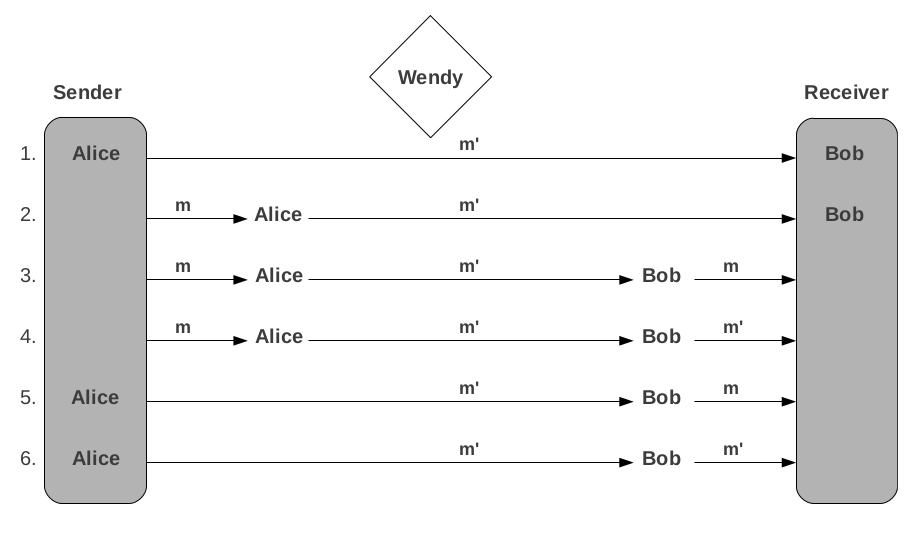
\includegraphics[width=0.8\textwidth]{communicationScenarios}
\caption{Communication Scenarios}
\label{fig:commScenarios}
\end{center}
\end{figure}

The six scenarios depicts different positions of Bob and Alice in the communication model, and the way the cover traffic (m) is manipulated by the covert channel (m\textprime).\\
The first scenario is the simplest one, it 
involves a communication between Bob and Alice, where Alice use directly the covert channel and insert the manipulated message, which is directed to Bob, the receiver. The remaining scenarios explores different 
combinations, depending on the behavior and identity of the sender, i.e. if Alice is the sender and introduces a manipulated message in the channel or Alice modifies an existing and legitimate one, or on the behavior and 
identity of the receiver, i.e. whether Bob is the receiver or, where he is not, if he restores or not the original message after reception.\\

``In these scenarios, Wendy always should be positioned between Alice and Bob so that she can monitor m\textprime\hspace{2pt} traffic. Were she positioned differently, and were unable to see m\textprime, her presence would be 
irrelevant to the covert communication''.\\
For the scope of this research, it is assumed that the sender can control the covert channel and insert directly the manipulated message. This reduction in scope, with respect to Lewandowski's study, is justified by the 
limitation in time, and by the simplicity of the network topology used for the experiment, that will be highlighted later in next chapters. However, it is worth saying that for an exhaustive testing of ICMPv6, related to 
covert channels, there are interesting implications to analyze inside the other scenarios, like the ability to preserve the covert channel in situations where Alice must modify the original message of the sender, or Bob 
must restore the original message before forwarding it to the legitimate receiver.\\
This assumption, however, has some implications:\\
``Alice can modify the traffic to a greater degree, since Bob does not necessarily expect the traffic to be meaningful and perhaps not even valid. On the other hand, if Alice and Bob use their own traffic to provide 
cover, they run a greater risk of exposure as they are openly communicating''.\\
Furthermore, in this research, it is assumed that both the sender and the receiver are the same subject.\\

Another topic to take into consideration, which relates to the behavior of the active warden, is the system and semantics preservation. The concepts have been applied first to preserve steganography
\footnote{``The art or practice of concealing a message, image, or file within another message, image, or file'', \url{http://www.merriam-webster.com/dictionary/steganography}, accessed 24.3.2016}\cite{lucena2}, but 
``the definitions can be applied to covert channels as well''\cite{netaware}.

\textbf{System Preservation} ``guarantees that the stegomessage is well formed within the rules of the protocol; the actual meaning of the stegomessage may be different than the original cover''\cite{lucena2}\\
\textbf{Semantic Preservation} ``means that, as observed at a point along the message’s path through the network, the stegomessage has the same meaning as the original cover''\cite{lucena2}\\

In the context of covert channels, ``the property of syntax preservation determines whether the modified traffic m\textprime\hspace{2pt}adheres to the protocol syntax. On the other hand, the property of semantics 
preservation guarantees that the meaning of modified traffic m\textprime\hspace{2pt}is the same as the original traffic m, or in other words that covert channel communication performed by Alice and Bob does not alter the 
meaning of cover traffic''.\\
The above concepts acquire more relevance in a complex topology scheme, where an IPv6 packet must eventually traverse multiple wardens. Lewandowski's work defines the concept of ``location-based syntax and semantics 
preservation'', which is useful to differentiate between nodes, along the path, ``performing distinct functions'' and with ``multiple levels of protocol knowledge and understanding''. Each node, with a particular function 
in the network, may behave differently with respect to the packet in travel, and ``as a result, a modified traffic’s syntax or semantics might be deemed correct by an IPv6 node with limited protocol knowledge while at 
the same time be rejected by a more knowledgeable node''.\\
This concepts will assume a particular relevance for this research when building the experiment. As it has been said before, it is important not only to understand the ICMPv6 protocol by itself, but also its relationship 
with devices like firewalls (the active warden) and the different configurations which produce different scenarios. Each configuration may lead to a different knowledge and understanding of the protocol by the node, which 
may affect the ability to preserve the covert channel, and must be taken into consideration. For example, an ``interesting case is presented by protocol’s reserved fields. Since their value is fixed (usually zeroed), and 
it is supposed to be ignored by the receiver, they do not carry any meaning and modifying such field does not alter packet’s semantics. If the modification in question avoids changing packet’s syntax as well, the 
reserved field is ideal for the purpose of embedding covert messages. And indeed, many network covert channel investigations focus on network protocol’s reserved fields and find them useful for covert communication''.
Therefor, choosing a different configuration for the device, a firewall or router, may affect the level of knowledge of the protocol of that device, and the ability to preserve the covert channel. Or, in the other way, 
each scenario may produce different behaviors with the presence of a covert channel, and allow to assess a particular configuration and its ability to prevent it.\\
Indeed, ``the objective of covert channel participants is to conduct their communication in such way that the necessary modifications of the cover traffic are always syntax and semantics preserving \textit{with respect} 
to network nodes along the communication’s path''.

\textbf{Analyzed RFCs}\\

The following table shows the list of protocols and associated RFC from Lewandowski's study that are in scope with this research. 
\vspace{15pt}
\begin{savenotes}
\begin{table}[h]
\centering
%\vspace{5pt}
%{\setlength{\extrarowheight}{10pt}
\begin{tabular}{|C{8.5cm}|C{4.5cm}|}
\rowcolor{darkblue}
\hline
%\multicolumn{4}{ |l| }{\textbf{Use Case:} Ensure authenticity of canceling}\\
Protocol&RFC\\
\hline
\rowcolor{lightblue}
IPv6 \footnote{RFC2460 is only partially in scope with this research, but it is worth to mention it because in ICMPv6 specification there are frequently references to IPv6 fields, like source and destination addresses}&RFC2460\cite{rfc2460}\\
\hline
\rowcolor{lightblue}
ICMPv6&RFC4443\cite{rfc4443}\\
\hline
\rowcolor{lightblue}
Neighbor Discovery (ND) for IPv6&RFC4861\cite{rfc4861}\\
\hline
\end{tabular}
\caption{Investigated Protocols}
\label{table:protocolsInScope}
\end{table}
\end{savenotes}

\textbf{Properties of Covert Channels}\\

Lewandowski's study proposed six properties of covert channels which are important for the investigation. In this research, given its scope, two of them have been considered:
\begin{itemize}
 \item ``degree of packet alteration – syntax- and semantics-preservation level of altered packets''. Since each configuration can have different syntax- and semantics-preservation level, it is important to test each 
 covert channel against each configuration, to assess both the warden configuration and the covert channel in this particular scenario.
 \item ``channel bandwidth – amount of data that can be transfered in given covert channel per packet of cover traffic''. This property does not affect the existence of the covert channel, but its ability to be preserved 
 for a longer period. Depending on the bandwidth, a covert channel may be useful, from attacker perspective, only in situations with a low amount of data to be exfiltrated, or when it is possible to insert a delay in the 
 transmission to avoid suspicion on the traffic.
\end{itemize}

Lewandowski observed that some of the considered protocols, Neighbor Discovering is an example of them, ``are designed for operation on a single network segment. In consequence, any covert channel using these protocols 
as a cover will be similarly limited in its range'', and that ``the communication can be easily defeated by simple address-based filtering mechanism''.\\
This research, even though the observation may be correct,  will not consider its assumption. The reason is given, as stated before, by the fact that it is important to consider also the actual transition period, where 
the two protocol, IPv4 and IPv6, cohexist in many configurations. This scenario implies that both networks are in place, but the active warden is configured to inspect only IPv4-related protocols, thus with a low level of 
syntax and semantics preservation knowledge, and any IPv6 packet will transit without deep inspection. For the same reason, an address-based filtering mechanism for IPv6 would probably not be in place. Another aspect, 
still related to the active warden, is the direction of the communication, from the inside to the outside: since it is considered a communication from a trusted to an untrusted network, the default configuration may 
allow the traffic without restrictions.



\pagebreak

%------------------------------METHODOLOGY-----------------------------------
\section{Methodology}
\label{sec:3}

\pagebreak

%------------------------------IMPLEMENTATION-----------------------------------
\section{Implementation}
\label{sec:4}

\pagebreak

%------------------------------EXPERIMENT-----------------------------------
\section{Experiment}
\label{sec:5}

\pagebreak

%------------------------------RESULTS-----------------------------------
\section{Results}
\label{sec:6}

\pagebreak

%------------------------------CONCLUSIONS-----------------------------------
\section{Conclusions}
\label{sec:7}

\pagebreak

%------------------------------REFERENCES-----------------------------------

\addcontentsline{toc}{section}{References}


\bibliographystyle{IEEEtran}
\bibliography{bibi.bib}


\pagebreak

%-----------------------------APPENDIX--------------------------------
\section*{Appendix 1 - [Title]}
%\label{Appendix 1}
\addcontentsline{toc}{section}{Appendix 1}

\end{document}
